\documentclass[12pt]{article}
\usepackage[top=1in, bottom=1in, left=1in, right=1in]{geometry}
\usepackage[justification=centering]{caption}
\usepackage{graphicx}
\usepackage{listings}
\usepackage{color}
\usepackage{indentfirst}
\usepackage{hyperref}
\usepackage{siunitx}
\usepackage{float}

\lstset{ %
	%language=C,                % choose the language of the code
	basicstyle=\scriptsize,       % the size of the fonts that are used for the code
	                  % how far the line-numbers are from the code
	backgroundcolor=\color{white},  % choose the background color. You must add \usepackage{color}
	showspaces=false,               % show spaces adding particular underscores
	showstringspaces=false,         % underline spaces within strings
	showtabs=false,                 % show tabs within strings adding particular underscores
	%frame=single,           % adds a frame around the code
	tabsize=2,          % sets default tabsize to 2 spaces
	captionpos=b,           % sets the caption-position to bottom
	breaklines=true,        % sets automatic line breaking
	breakatwhitespace=false,    % sets if automatic breaks should only happen at whitespace
	escapeinside={\%*}{*)}          % if you want to add a comment within your code
}

\newcommand{\uz}{UART0}
\newcommand{\uo}{UART1}

\begin{document}
\title{Microprocessor Systems\\ Lab 3: Asynchronous \&\ Synchronous Serial Communications }
\author{Nick Choi \and Samuel Deslandes}
\date{10/17/16}
\maketitle
\pagebreak
\section{Introduction}

The overall goal of this lab is to become familiar with configuring the UART and SPI serial communication protocols on the 8051 and utilizing their respective interrupts to perform terminal operations. 

The lab is divided into three sections. In the first section, a C program is created to configure both UART0 and UART1 on the 8051 to react to keyboard presses. The code constantly polls both of the ports to check whether a keyboard character has been entered into the terminal. Once a character is pressed, the program will echo the character back to the terminal on both UART0 and UART1. If the entered character is an  \textless ESC\textgreater\ key, the program displays a brief message and stops the program on both UARTs. Unlike past labs, the getchar() function could not be used to check whether a keyboard button was pressed because it would only check UART0. 

In the second section, the program’s logic changed so that interrupts would be used rather than polling. Additionally, the program needed to be altered so that two 8051’s could communicate through their UART1 connections.

In the third section, a new C program is written to echo characters using the 8051\textquoteright s SPI protocol. Whenever a character is entered on the 8051’s UART0, it will be echoed to the terminal through the 8051\textquoteright s SPI0. A loopback wire is used to connect the MISO and MOSI pins to verify that the SPI configuration was successful. Once the SPI0 is configured correctly, the code is modified again so that the 8051 can communicate with a 68HC11 via SPI0. The 8051 functions as the master device and the 68HC11 functions as the slave device. 
\section{Methods}
\subsection{Software}
The code for parts 1, 2 and 3 can be found in the appendix below. All code was uploaded and run on the 8051 through the programming/debugging USB port. Code for the 68HC11 was uploaded via the terminal interface. 	

\subsubsection{Part 1}
The purpose of the C program for the first section of the lab was to write a procedure that would monitor the UART0 and UART1 serial ports continuously and echo a character received on one port to the other. For this section of the lab, this was accomplished by polling the receive interrupt flags RI0 and RI1 for UART0 and UART1 respectively. 

Since this lab uses both UART0 and UART1, both ports must be enabled on the crossbar. The enable bit for UART0 can be found on the XBR0 SFR and the enable bit for UART1 can be found on the XBR1 SFR. As always, the crossbar enable bit in XBR2 must be set. UART0 was configured to be in mode 1 (8-bit UART with variable baud rate) and to use Timer2 to generate a baud rate of \si{9600}{bps}. UART0 configuration can be set in the SSTA0 and SCON0 SFRs. Timer2 was configured to be in auto-reload mode and use SYSCLK as a base. These settings can be found in the TMR2CN and TMR2CF SRFs. To count to 9600, the reload value must be set to \texttt{0xFEBC}. This was calculated as follows:\\
\begin{equation}
	\mathtt{Mode1\_BaudRate} = \frac{\mathtt{SYSCLK}}{16*(65536-\mathtt{ReloadValue})}
\end{equation}\\
For a desired baud rate of 9600 and SYSCLK of \si{49,766,400}{Hz}, this comes out to:\\
\begin{equation}
9600= \frac{49766400}{16*(65536-\mathtt{ReloadValue})}
\end{equation}
\begin{equation}
\mathtt{ReloadValue} = 65212
\end{equation}
This is equivalent to \texttt{0xFEBC} in hex.

UART1 was similarly configured, but used Timer1 to generate a baud rate of \si{115200}{bps}. UART1 can be configured in the SCON1 SFR. Timer1 was set to be an 8-bit counter with auto-reload, and use SYSCLK as a base; this configuration can be set in the TMOD SFR. The Timer1 reload value should be set as \texttt{0xE5}. This was calculated as shown below:\\ 
\begin{equation}
\mathtt{Mode1\_BaudRate} = \frac{\mathtt{SYSCLK}}{16*(256-\mathtt{ReloadValue})}
\end{equation}
\begin{equation}
\mathtt{ReloadValue} = 229
\end{equation}\\
This is equivalent to \texttt{0xE5} in hex.

When configuring both UARTs, the receive enable bits must be set in the SCON SFRs and the timers need to be started. In the P0MDOUT SFR, the TX pins (P0.0, P0.2) should be set as push-pull for outputs, and the RX pins (P0.1, P0.3) as open-drain for inputs. Additionally, in the P0 SFR set the inputs (RX pins) for high impedance. 

The main routine of this program consists of two sub-routines `checkSBUF()' and `echo()' which are run in an infinite loop. The `checkSBUF()' function continuously polls RI0 and RI1, and returns the value stored in the UART data register when one of the flags is set. The UART data register (SBUFn) is used for both the transmit and the receive buffer. When data is read from SBUF, as is the case for the `checkSBUF()' function, it comes from the receive buffer. When data is written to SBUF, it goes to the transmit buffer where it is held until a full byte has been written. At this point, the data transmission will begin. The returned value from `checkSBUF()' is then passed into the `echo()' function, where it is loaded into both SBUF0 and SBUF1 for transmission to both terminals. Recall that SBUF0 and SBUF1 are on different pages, and that SFRPAGE should be changed accordingly. 

\subsubsection{Part 2}
This section of the lab was divided into two parts.
The task for the first part was similar to that of section 1, however rather than polling, interrupts were used. The second part involved connecting the UART1s of two 8051s so that whenever a key is pressed on either UART0, the character will be displayed on both of the boards\textquoteright s UART0s. The initial configurations were all the same as section 1, with the addition of having to set the global interrupt enable bit (EA), as well as the individual UART0 and UART1 interrupt enable bits which can be found on the IE and EIE2 SFRs respectively. With these bits set, whenever the transmit interrupt flags (TIn) or receive interrupt flags (RIn) are set, the CPU vectors to the appropriate interrupt service routine (ISR); these flags must be cleared manually by the software. The UART0 interrupt has a priority level of 4, while the \uo\ interrupt has a priority of 20. One thing to keep in mind is that while UART0 interrupts are enabled, unless the UART0 and UART1 interrupt priorities are swapped, UART1 will not receive any interrupts. Since both receiving and transmitting will trigger an interrupt, the ISR must poll each flag to verify the source of the interrupt. 

For part 1 of this section of the lab, the main function will only check if the command to end the program had been sent; everything else was handled in the ISRs. The \uz\ ISR checks if the source of the interrupt was a receive by checking if RI0 has been set. If so, it is cleared and the `echo()' subroutine is called. After this, \uz\ interrupts are temporarily disabled to allow \uo\ interrupts to go though. The \uo\ ISR has the same routine, however rather than disabling \uz\ interrupts, it re-enables them.

The program for part 2 was slightly differently, with the main routine now continuously polling two flags `UART0\_flag' and `UART1\_flag', which will be set in the ISRs of UART0 and UART1 respectively. The `echo()' function is also used for this part of the lab, but with the slight modification of disabling \uz\ interrupts before loading data into the SBUF registers. The \uz\ ISR checks whether the source of the interrupt is a receive; if it is, it clears RI0, reads SBUF0 into a global variable, and sets the \uz\_flag. The \uo\ ISR does the same, but enables \uz\ interrupts at the end of the ISR. 

In the main routine, once the \uz\_flag has been set, the program calls the `echo()' function and clears the flag. If the \uo\_flag has been set, the program disables \uz\ interrupts, transmits the character to \uz\ via the SBUF0 register, re-enables \uz\ interrupts and clears the flag. In this case, the character is sent only to \uz\ rather than being echoed to both ports to avoid a feedback loop of infinite transmissions between the two microcontrollers.

In order to allow interrupts on \uo\ to go through, in the main routine there is a brief period of time in which \uz\ is disable. This small window was implemented by incrementing a variable to 255 in a for loop.


\subsubsection{Part 3}
The third section of this lab deals with the serial peripheral interface bus (SPI), a synchronous serial communication interface. The goal of this section was to communicate with the 68HC11 as a slave device, and use it to echo back any characters that get sent to it. Although the primary focus of this lab is SPI, UART0 is also used to send data to the terminal. As was the case with UART, SPI must also be enabled on the crossbar to function; it's enable bit can be found on XBR0. The relevant configuration SFRs for SPI are SPI0CFG, SPI0CN, and SPI0CKR. In SPI0CFG, master mode is enabled so that the 8051 acts as the master device. In the SPI0CN register, enable SPI0, and set it to operate in 4-wire single master mode. The SPI0CKR register stores data pertaining to SPI clock rate, which can be calculated as follows:\\
\begin{equation}
SCK = \frac{SYSCLK}{2\times(SPI0CKR+1)}
\end{equation}\\
Setting SPI0CKR to \texttt{0x18} with a SYSCLK of 49,766,400 results in a SCK of \si{995,328}{Hz}. For SPI communication, in the P0MDOUT SFR, the SCK, MOSI, and NSS pins (P0.2, P0.4, P0.5 respectively) must be set to push-pull.

The program for this section used 3 sub-routines: `SPI0\_READ()' handles receiving data from the slave device and outputting it to the terminal, `SPI0\_WRITE()' handles receiving user input and sending that data to a slave device, and `write\_dummy()' sends a byte of garbage data (a dummy) to the slave device. The main routine simply waits for user input by polling RI0, and when set, clears the flag and calls the  `SPI0\_WRITE()' and `SPI0\_READ()' functions.

The `write\_dummy()' function first selects the slave by clearing NSSMD0. It then checks to make sure that SPI is not busy, then clears SPIF and writes a byte of data (\texttt{0xFE} in this case) to the SPI data register SPI0DAT. Like the UART data register (SBUF), SPI0DAT is used both to receive and transmit. Checking that the SPI is not busy with a transmission can be done by monitoring bit 7 of the SPI0CFG register. SPIF is the SPI interrupt flag, which is set at the end of a data transfer. Like RIn and TIn, this flag must be cleared manually. 

The `SPI0\_WRITE()' function starts by loading the data in SBUF0 into a variable. It then selects the slave, ensures that SPI is not busy, clears SPIF, and loads the variable into SPI0DAT to be sent to the slave. It then waits for the transmission to end and clears SPIF. Because the slave device contains a second shift register, the echoed response will be delayed by one transmission. This is why dummy bytes must be read and written in between every actual read and write. The next step in the `SPI0\_WRITE()' routine is to read the dummy byte, which is done by selecting the slave and moving the dummy byte out of SPI0DAT. This program will output the dummy char to the terminal. After reading the dummy char, the input character (received on UART0) is displayed on the terminal and the `write\_dummy()' function is called. The `SPI0\_READ()' function follows the same procedure as reading the dummy byte.

The display is formatted using ANSI escape sequences to split the screen horizontally, with the top half used to display the input received on UART0, and the bottom half for the echoed character (received on the MISO pin of SPI). In order to make the two halves scroll independently, the scroll area must be redefined to the half being printed to before each print. A for loop was used to move the cursor to the appropriate position. All of these features were implemented through ANSI escape sequences.
\subsection{Hardware}
The hardware for section 1 involved connecting a DB9 adapter to be used at the UART1 port. A schematic for this can be viewed in the appendix below. The TD pin on the DB9 was connected to the input of a hex inverter, with the output connected to the RX1 pin of UART1 (P0.3). The TX1 pin (P0.2) was connected to the input of an inverter, with the output connected to the RD pin on the DB9. In order to establish a common ground between the adapter and the microcontroller, the ground pin on the DB9 was connected to pin 1 on the 60 pin bus (DGND), which was connected to the ground on the power supply used. 
 
Section 2 called for connecting the UART1s of two microcontrollers. This was done by connecting the TX1 pin of one 8051 to the RX1 pin of the other, and vice versa for the RX1 pin. A diagram of this can also be found in the appendix below.

In section 3, the 68HC11 EVB was used as a SPI slave device. It was connected to the 8051 by connecting the MISO pins (pin 22 on 68HC11 to P0.3 of 8051), the MOSI pins (pin 23 on 68HC11 to P0.4 of 8051), the SCK pins (pin 24 on 68HC11 to P0.2 of 8051), the SS* pin on the 68HC11 to the NSS pin on the 8051 (pin 24 on 68HC11 to P0.5 of 8051), and establishing a common ground between the two devices (pin 1 on both 60 pin buses). The schematic for this can be viewed in the appendix section below. 
\section{Results}

By completing section one of the lab, a functioning C program was produced to echo characters between the 8051’s UART0 and UART1 ports via polling. After completing section two of the lab, a C program was developed to echo characters between two 8051s’ UART ports. The UART0 ports were used to take in the keyboard presses and the UART1 ports were used to communicate between the two processors. By completing section three of the lab, a C program was created to use the 8051’s SPI0 port to echo characters back and forth with an 68HC11. 


\section{Conclusion}

The end results of the lab generally matched with the initial goals however there were numerous instances where the system did not behave as expected. During section 2 and 3 of the lab, a lot of time was spent testing and debugging the C programs to control the serial communication ports. An enhancement was added to section two of the lab so that the characters echoed by both UARTs would scroll on the screen in two separate scrolling areas. 
If more time was given to complete this lab assignment, additional enhancements would be added to section 3 of the lab so that the slave would react to certain keypresses. This would increase the functionality of the SPI0 communication and would make the program more interactive for the user. 




\pagebreak
\section{Appendices}
\subsection{Modified putget.h}
	\lstinputlisting{putget.h}
\subsection{Part 1}
	\subsubsection{Circuit Schematic for section 1}
		\begin{figure}[H]
			\centering
			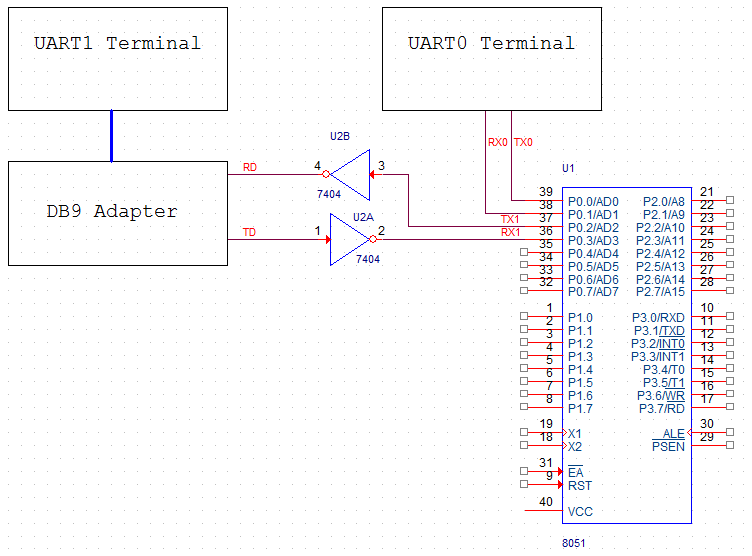
\includegraphics[width=\textwidth]{Part1Schematic.png}
			\caption{Circuit schematic for part 1}
			\label{schematic1}
		\end{figure} 
		\pagebreak
	\subsubsection{Code for part 1}
		\lstinputlisting{part1.c}
\subsection{Part 2}
	\subsubsection{Circuit Schematic for section 2}
		\begin{figure}[H]
			\centering
			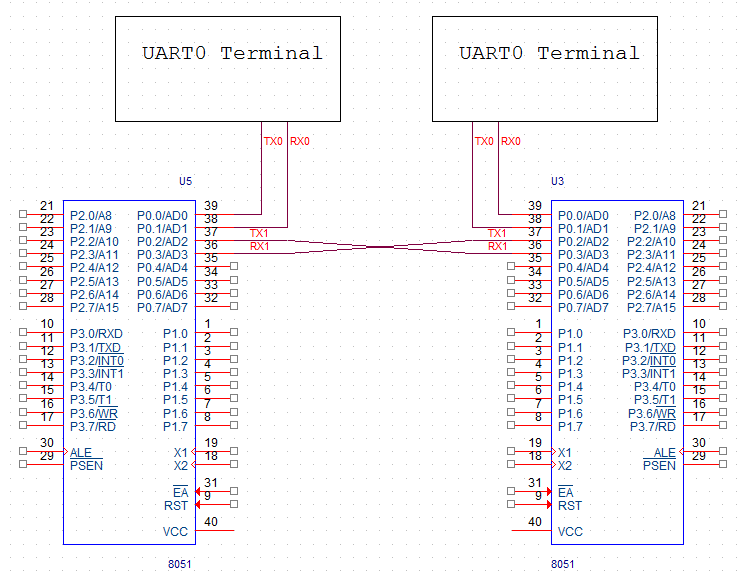
\includegraphics[width=\textwidth]{Part2Schematic.png}
			\caption{Circuit schematic for part 2}
			\label{schematic2}
		\end{figure} 
		\pagebreak
	\subsubsection{Code for part 2}
		\lstinputlisting{part2-2v2_publish.c}	

%\pagebreak
\subsection{Part 3}
	\subsubsection{Circuit Schematic for section 2}
		\begin{figure}[H]
			\centering
			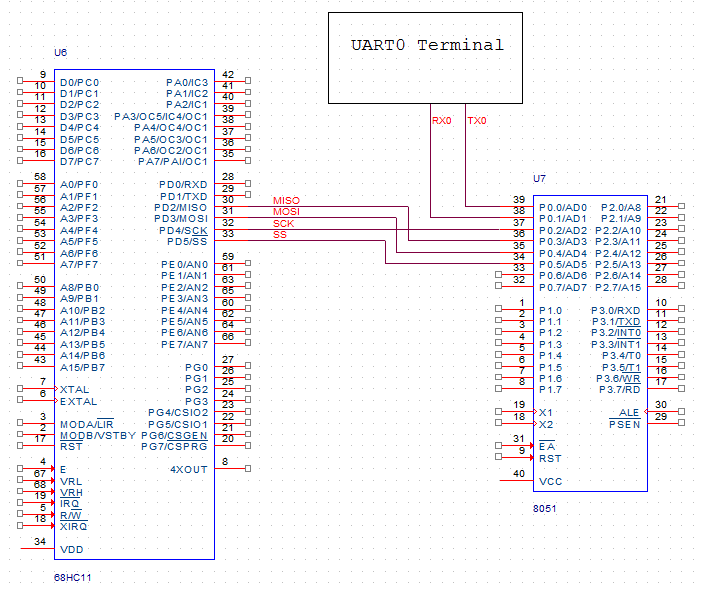
\includegraphics[width=\textwidth]{Part3Schematic.png}
			\caption{Circuit schematic for part 3}
			\label{schematic3}
		\end{figure}
	\pagebreak
	\subsubsection{Code for part 3}
		\lstinputlisting{part3-2_publish.c}
	
\section{References} 
\noindent
``MPS Lab 3," in RPI ECSE Department, 2016. [Online]. Available: \url{http://www.rpi.edu/dept/ecse/mps/MPS_Lab_Ex3-Serial.pdf}. Accessed: Oct. 16, 2016.\\
\newline\noindent
``C8051 Manual," in RPI ECSE Department, 1.4 ed., 2005. [Online]. Available: \url{https://www.ecse.rpi.edu/courses/CStudio/Silabs/C8051F12x-13x.pdf}. Accessed: Oct. 16, 2016.








\end{document}